The field of data visualization is lacking open tools that support easily developing and using production quality interactive visualizations. While powerful visualization and data analysis technologies exist such as Tableau \cite{hanrahan2007visual}, Spotfire \cite{spotfire}, SAS Visual Analytics \cite{sas2012sas} and Wolfram Alpha \cite{wolframAlpha}, they cannot be freely leveraged as tools by researchers or components for application developers due to their proprietary nature. The primary open source tool for Web-based data visualization is D3.js \cite{d3}, a JavaScript library that provides low level primitives for constructing interactive visualizations. Creating visualizations using D3 typically involves copying one of the many visualization examples available, then tailoring it to work with the application-specific tasks and data at hand. Though there have been many attempts at creating generalized visualization environments using D3, none of them rival the power of commercial visualization packages.

Open Source projects often serve as a bridge between academic theory and professional practice. For example, Hadoop has made parallel computation more accessible, and PostgreSQL has served as a platform to bring advanced database techniques into practice. D3 has served as a bridge between data visualization theory and practice largely via the self-contained examples found in the D3 Example Gallery \cite{d3examples}. However, most D3 examples are not reusable solutions but rather one-off implementations tailored to a specific data set and task. There is a need for an approach to generalizing D3 examples that results in reusable interactive visualization components. Chapter 1, ``Reactive Visualizations'' introduces a solution for generalizing existing visualization examples using concepts from functional reactive programming and the Model View Controller paradigm.

Some of the most common requirements of visualization applications today are that they have multiple linked views, can be developed collaboratively, and can be easily shared. Having linked views means that interactions in one visualization cause some change in other visualizations on the page. Being developed collaboratively means that many people in a group are all able to make changes that can subsequently be leveraged by others in future work. Being easily shared means that the resulting visualizations can be embedded within presentations, reports, or third party Web sites. Chapter 2 ``Collaborative Visual Data Exploration'' discusses an approach to collaboration, history and linked views that leverages reactive visualizations.

Much of the work of a data scientist or analyst is dedicated to curating and transforming data such that they can perform their analyses. Many data sets, in aggregated form, can be transformed into data cube using binned aggregation \cite{liu2013immens}. Data cubes are data structures based on dimensions and measures. Dimensions contain (potentially hierarchical) sets of distinct entities or concepts. Measures are quantitative properties that represent aggregates (such as sum or average). Many data cube dimensions, such as Space, Time, Gender and Industry, are ``universal'' in that they transcend any single data set. Observations (sometimes called facts) within a data cube assign concrete numeric values to measures of the data cube corresponding to the cartesian product of members from each dimension. These dimensions may be referenced by different data sets using different identifiers, and data sets may present the same measure with a different scale or attribute naming convention. Chapter 3 ``The Universal Data Cube'' introduces a collection of data structures and algorithms for integrating and visualizing many data sets.

Taken together, the contributions of this dissertation make inroads toward an open platform for complex data visualization. The hope is that these technologies can continue to evolve with support from the global Open Source community and can evolve into a mature platform for advanced data visualization applications.

\section{Vision}
The envisioned data representation and visualization framework can serve as a digital telescope into the universe of phenomena on Earth via publicly available data. For example, consider data sources such as the United Nations, the US Census, the US Bureau of Labor Statistics, or the US Centers for Disease Control. These organizations and hundreds of others around the world provide publicly available data about various topics including population statistics, public health, distribution of wealth, quality of life, economics, the environment, and many others. By unifying these data sources and providing users with tools to explore them visually, a deeper understanding of the world can be gleaned by anyone through the lens of data.

There is immense potential value in data that is not being realized. The ability to visually explore data lends itself to applications in education, journalism, and public policy. Especially in the era of ``Big Data,'' it is increasingly valuable for organizations and individuals to have the ability to analyze large quantities of data that come from various sources and vary across time, space, and other dimensions. In addition, publicly available data can provide context for business-centric, proprietary data analysis activities.

\begin{figure}
  \centering
  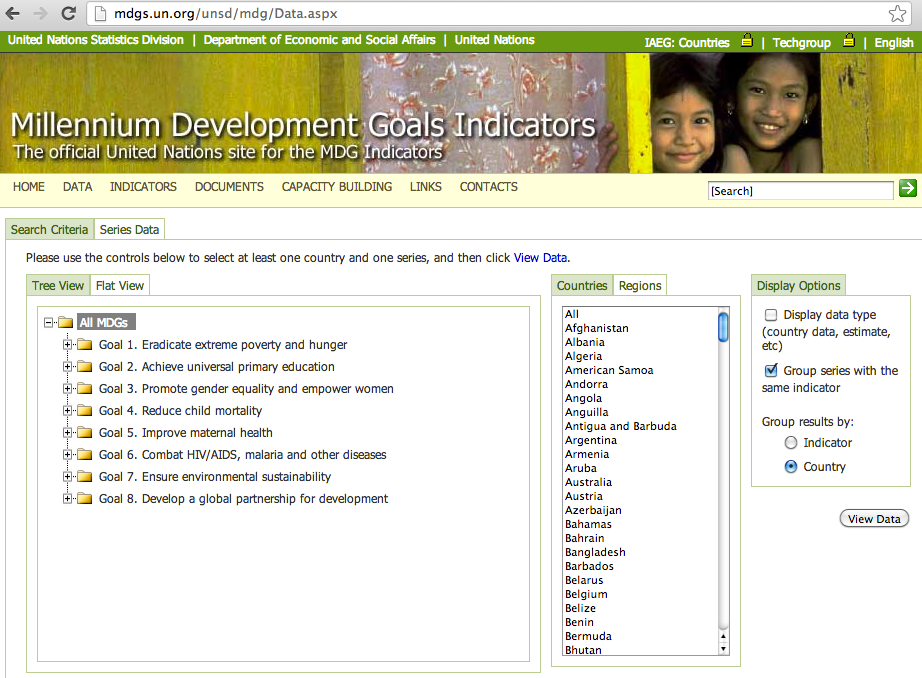
\includegraphics[width=\figureWidth]{figs/MDGInterface.png}
  \caption[Millennium Development Goals User Interface.]
   {The Web-based interface provided for navigating the United Nations Millennium Development Goals Indicator data sets \cite{mdgDataUI}. This is one example of the variety of formats and protocols used for making data available on the Web.}
  \label{fig:MDGInterface}
\end{figure}

\begin{figure}
  \centering
  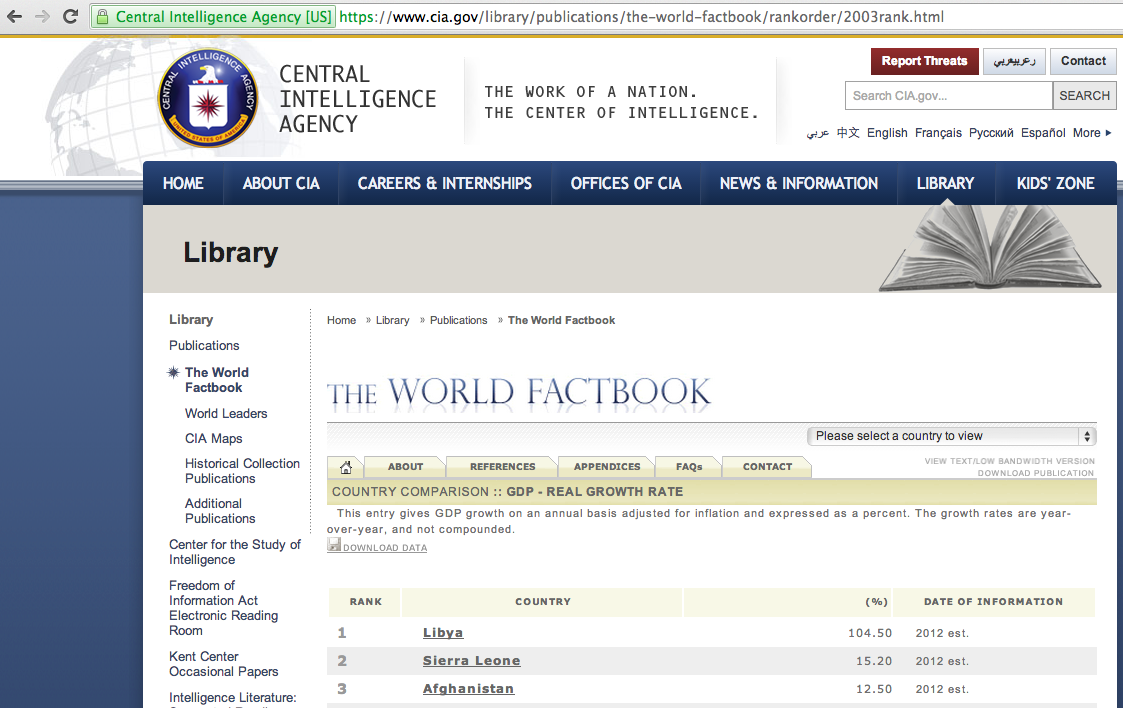
\includegraphics[width=\figureWidth]{figs/CIAWorldFactbook.png}
  \caption[CIA World Factbook User Interface.]
    {The Web-based interface for downloading data from the CIA World Factbook \cite{ciaWorldFactbookData}. A data download link is provided that yields a text file using a nonstandard table format. This is a second example of the variety of formats and protocols used for making data available on the Web.}
  \label{fig:ciaWorldFactbook}
\end{figure}

\begin{figure}[h!]
  \centering
  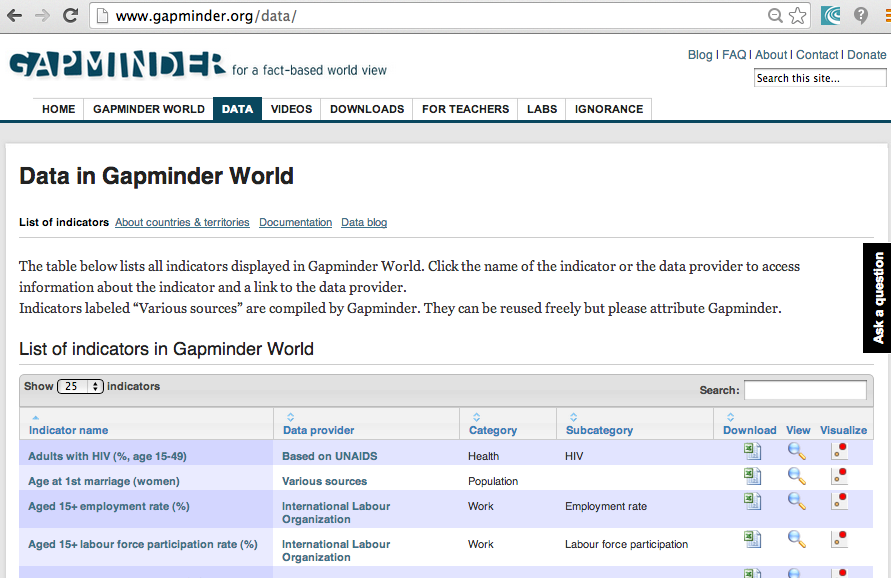
\includegraphics[width=\figureWidth]{figs/gapminderData.png}
  \caption[GapMinder Data Access User Interface.]
    {The Web-based interface for downloading data harvested by the GapMinder project \cite{gapminderData}. A data download link is provided for each indicator that yields an Excel spreadsheet hosted using Google Docs.}
  \label{fig:gapminderData}
\end{figure}

\begin{figure}[h!]
  \centering
  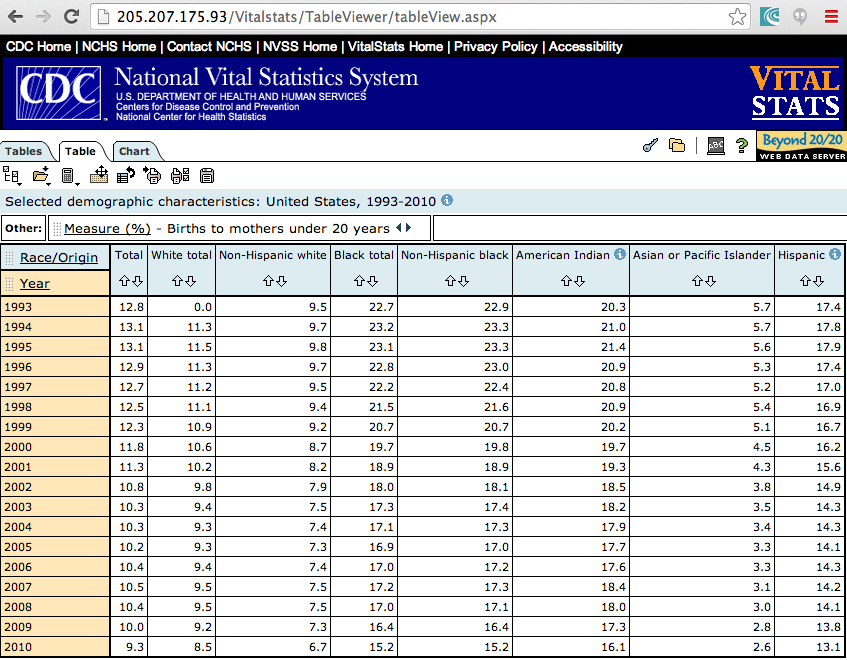
\includegraphics[width=\figureWidth]{figs/CDCVitalStatsUI.png}
  \caption[CDC Vital Statistics User Interface.]
    {The Web-based pivot table user interface for downloading data from the US Centers for Disease Control about births to mothers under age 20 by demographic and year \cite{CDCVitalStatsUI}. The product powering this interface is the Beyond 20/20 Web Data Server \cite{beyond2020webDataServer}. In this interface a ``download'' button is provided that yields data in CSV (Comma Separated Value) format.}
  \label{fig:CDCVitalStatsUI}
\end{figure}

\begin{figure}
  \centering
  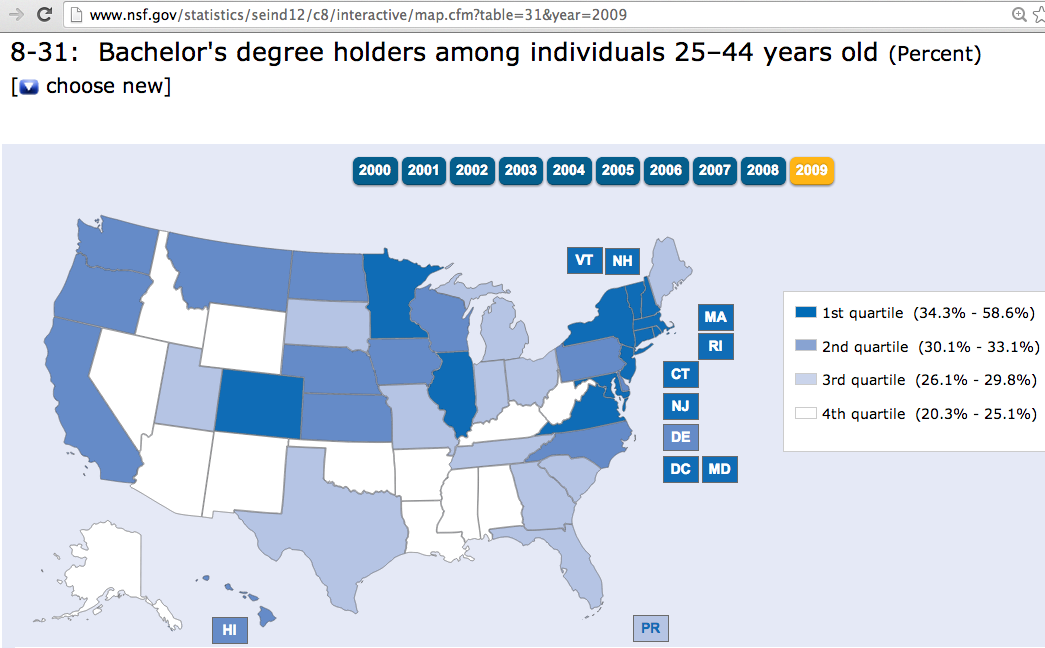
\includegraphics[width=\figureWidth]{figs/nsfBachelorsDegrees.png}
  \caption[NSF Bachelors Degrees Statistics Choropleth Map.]
    {An interactive visualization of bachelors degree statistics provided by the National Science Foundation site \cite{nsfBachelorsDegrees}. This is an example of an extremely limited visualization tool provided along with a data set.}
  \label{fig:nsfBachelorsDegrees}
\end{figure}

While publicly available data sets are available on the Web, it is difficult to realize their full value in practice. The difficulty stems from the fact that they are made available using numerous formats and protocols. The heterogeneity of formats and protocols used makes it difficult to combine and analyze data sets together and hinders the development of analysis and visualization tools. For example, some data sets are made available as CSV files, Excel spreadsheets (as shown in figure \ref{fig:unPopExcel}), or must be navigated using a Web-based user interface (as shown in figures \ref{fig:MDGInterface}, \ref{fig:ciaWorldFactbook}, \ref{fig:gapminderData} and \ref{fig:CDCVitalStatsUI}).

Sometimes visualization interfaces are provided for data published online, such as in figure \ref{fig:nsfBachelorsDegrees}, but these tools are typically extremely limited in scope and hard-coded to the data set at hand.  With the tools available today such as D3.js, creation of Web-based interactive data visualizations involves hard coding one-off projects to a particular data set. Ideally, anyone should be able to apply interactive visualization techniques to data easily. This dissertation focuses on the challenges in making this a reality and offers a solution based on the data cube concept. The proposed framework reduces the effort required to create Web-based data visualizations by linking reusable visualization components with data sets within the proposed data representation framework, which is based on the data cube model.

Public data tends to be particularly well suited to the data cube model because it typically contains measures about people (or byproducts of human activities) distributed across time, space (geographic regions), and other dimensions such as gender or age range. For example, the data available in the GapMinder visualization tool contains measures (such as ``number of adults with HIV/AIDS'' and ``child mortality'') aggregated across countries and years \cite{gapminderData}. This partitioning of space into countries and time into years is one choice of levels in the space and time hierarchies, but the data cube model is more general in that it can support multiple levels of detail in both the Space dimension (e.g., Continents, Countries, States, Counties, and Metropolitan Areas) and the Time dimension (e.g., millennia, centuries, years, months, days, hours and minutes). Therefore, any data sets that contain measures (also called statistics, indicators, or metrics) aggregated along any resolution of time and space can be modeled as data cubes.

When multiple data sets are modeled as data cubes, they can be integrated into a single structure. Based on the common dimensions and measures shared between data sets, an integrated heterogeneous data cube structure can be created from an arbitrary number of data sets from multiple sources. Interactive visualization techniques can be applied to this integrated structure, yielding fundamentally new ways of exploring and presenting multiple data sets.

To motivate research in data cube integration and visualization, one must consider a larger picture. The data available today can paint a vivid picture of the world if it is exposed in a meaningful way. Data visualization augments human cognition by enabling users to glean knowledge from data using visual perception rather than detailed mental analysis \cite{card1999readings}. Data cubes provide a well structured, common representation that captures the essence of many data sets. Data visualization augments human cognition by offloading data analysis tasks to tasks of visual perception. The synthesis of data with visualization through data cubes can lead to a technology platform that changes the world by bringing the power of data visualization to the public.

\section{Challenges}
The main problem this work addresses is the gap between heterogeneous data sets and information visualization software. The reality of the current data visualization landscape contains many disparate data sets, data formats, visualization tools (specific implementations), and visualization techniques (abstract conceptual visualization approaches). The problem with this situation is that it requires an immense amount of manual work to establish a complete pipeline from any given data source to an instantiation of a visualization technique. This situation is summarized in figure \ref{fig:reality}.

\begin{figure}
  \centering
  
\includegraphics[height=2in]{figs/Reality.png}
  \caption[Fragmentation of Data and Visualization.]
   {The fragmentation of data and visualization. }
  \label{fig:reality}
\end{figure}

An ideal solution to this problem would allow any target data set to be visualized using any target visualization technique. For example, the task ``Visualize the US Census Population Statistics on a Choropleth Map'' should be possible to execute in a straightforward way, ideally by a simple process in which the target data set is selected (US Census Population Statistics), the target visualization technique is selected (Choropleth Map), and the mapping from the data set to the visualization technique is configured (total population maps to region color by a selected color scale). This ideal is summarized in figure \ref{fig:ideal}.

\begin{figure}
  \centering
  
\includegraphics[height=2in]{figs/Ideal.png}
  \caption[Bridging the Gulf between Data and Visualizations.]
   {Bridging the gulf between data and visualizations.}
  \label{fig:ideal}
\end{figure}

The proposed solution to address the gulf between data sets and visualization techniques involves the introduction of a generic and powerful intermediate data representation. The generic data representation should be capable of representing most data sets. For this the data cube concept was chosen as a foundation, as it captures the essential structure of many data sets. This solution is summarized in figure \ref{fig:solution}.

\begin{figure}
  \centering
  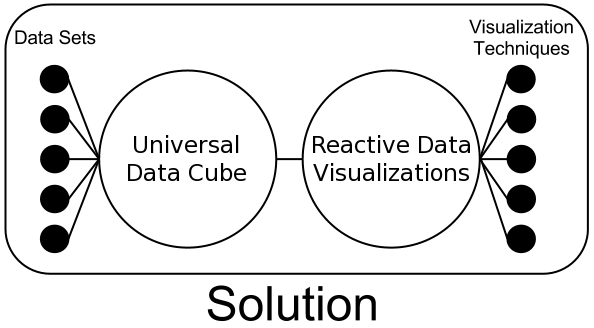
\includegraphics[height=2in]{figs/Solution.png}
  \caption[Introducing Intermediate Representations.]
   {Our proposed solution; introduce generic intermediate representations conducive to data visualization.}
  \label{fig:solution}
\end{figure}

\section{Application Areas}
Imagine what it would be like if any person could readily access or construct interactive visualizations of data. Interactive data visualization has relevance to many application areas including, but not limited to, education, journalism, and big data analytics.

Educational material is ripe with opportunity for augmentation by interactive visualizations. For example, consider the next generation of textbooks as eBooks running on tablets. Textbooks covering historical trends can use visualization to represent data about, for example, the distribution of various demographics across the Earth and how they have shifted over centuries. Economics courses could use interactive visualizations of global economic data to help students better understand socioeconomic dynamics. Environmental studies can include visualizations of data on climate and pollution. Medical studies can take advantage of public health data. There is no end to the potential applications of public data visualization in education.

Journalism requires an in-depth understanding of stories as they evolve. Public data can provide context for those stories, and interactive visualizations of relevant data can be placed in digital publications alongside article text. This places the power of interactive visualization in the hands of readers. Visualizations are already being used for this purpose today by publishers such as the New York Times and the Boston Globe \cite{royal2010journalist}.

Big data analytics is a fast growing area of active research and development. The proposed data modeling and visualization approach has relevance for big data analytics because the data cube construct is a particularly well suited structure for presenting summary queries executed across large distributed data stores. For example, Facebook developed a visualization system based on data cubes and interactive specification of slices \cite{facebookBigData}. In this system, a distributed in-memory database developed at Facebook is interactively queried based on user-defined filters that compute data cube aggregates of real-time data on demand. LinkedIn is taking a similar approach to present real-time aggregated data to users through visualizations \cite{linkedInBigData}.


%\TODO{Discuss apply(fn, args)}

%\TODO{Discuss !bool}

